\documentclass[11pt,a4paper,]{article}
\usepackage{lmodern}

\usepackage{amssymb,amsmath}
\usepackage{ifxetex,ifluatex}
\usepackage{fixltx2e} % provides \textsubscript
\ifnum 0\ifxetex 1\fi\ifluatex 1\fi=0 % if pdftex
  \usepackage[T1]{fontenc}
  \usepackage[utf8]{inputenc}
\else % if luatex or xelatex
  \usepackage{unicode-math}
  \defaultfontfeatures{Ligatures=TeX,Scale=MatchLowercase}
\fi
% use upquote if available, for straight quotes in verbatim environments
\IfFileExists{upquote.sty}{\usepackage{upquote}}{}
% use microtype if available
\IfFileExists{microtype.sty}{%
\usepackage[]{microtype}
\UseMicrotypeSet[protrusion]{basicmath} % disable protrusion for tt fonts
}{}
\PassOptionsToPackage{hyphens}{url} % url is loaded by hyperref
\usepackage[unicode=true]{hyperref}
\hypersetup{
            pdftitle={Predicting Critical Elements in Coal Mine Waste: A Machine Learning and Spatial Statistics Approach for a Low-Emission Future},
            pdfborder={0 0 0},
            breaklinks=true}
\urlstyle{same}  % don't use monospace font for urls
\usepackage{geometry}
\geometry{a4paper, centering, text={16cm,25cm}}
\usepackage[style=authoryear-comp,]{biblatex}
\addbibresource{references.bib}
\usepackage{longtable,booktabs}
% Fix footnotes in tables (requires footnote package)
\IfFileExists{footnote.sty}{\usepackage{footnote}\makesavenoteenv{long table}}{}
\usepackage{graphicx,grffile}
\makeatletter
\def\maxwidth{\ifdim\Gin@nat@width>\linewidth\linewidth\else\Gin@nat@width\fi}
\def\maxheight{\ifdim\Gin@nat@height>\textheight\textheight\else\Gin@nat@height\fi}
\makeatother
% Scale images if necessary, so that they will not overflow the page
% margins by default, and it is still possible to overwrite the defaults
% using explicit options in \includegraphics[width, height, ...]{}
\setkeys{Gin}{width=\maxwidth,height=\maxheight,keepaspectratio}
\IfFileExists{parskip.sty}{%
\usepackage{parskip}
}{% else
\setlength{\parindent}{0pt}
\setlength{\parskip}{6pt plus 2pt minus 1pt}
}
\setlength{\emergencystretch}{3em}  % prevent overfull lines
\providecommand{\tightlist}{%
  \setlength{\itemsep}{0pt}\setlength{\parskip}{0pt}}
\setcounter{secnumdepth}{0}

% set default figure placement to htbp
\makeatletter
\def\fps@figure{htbp}
\makeatother


\title{Predicting Critical Elements in Coal Mine Waste: A Machine Learning and Spatial Statistics Approach for a Low-Emission Future}

%% MONASH STUFF

%% CAPTIONS
\RequirePackage{caption}
\DeclareCaptionStyle{italic}[justification=centering]
 {labelfont={bf},textfont={it},labelsep=colon}
\captionsetup[figure]{style=italic,format=hang,singlelinecheck=true}
\captionsetup[table]{style=italic,format=hang,singlelinecheck=true}


%% FONT
\RequirePackage{bera}
\RequirePackage[charter,expert,sfscaled]{mathdesign}
\RequirePackage{fontawesome}

%% HEADERS AND FOOTERS
\RequirePackage{fancyhdr}
\pagestyle{fancy}
\rfoot{\Large\sffamily\raisebox{-0.1cm}{\textbf{\thepage}}}
\makeatletter
\lhead{\textsf{\expandafter{\@title}}}
\makeatother
\rhead{}
\cfoot{}
\setlength{\headheight}{15pt}
\renewcommand{\headrulewidth}{0.4pt}
\renewcommand{\footrulewidth}{0.4pt}
\fancypagestyle{plain}{%
\fancyhf{} % clear all header and footer fields
\fancyfoot[C]{\sffamily\thepage} % except the center
\renewcommand{\headrulewidth}{0pt}
\renewcommand{\footrulewidth}{0pt}}

%% MATHS
\RequirePackage{bm,amsmath}
\allowdisplaybreaks

%% GRAPHICS
\RequirePackage{graphicx}
\setcounter{topnumber}{2}
\setcounter{bottomnumber}{2}
\setcounter{totalnumber}{4}
\renewcommand{\topfraction}{0.85}
\renewcommand{\bottomfraction}{0.85}
\renewcommand{\textfraction}{0.15}
\renewcommand{\floatpagefraction}{0.8}


%\RequirePackage[section]{placeins}

%% SECTION TITLES


%% SECTION TITLES
\RequirePackage[compact,sf,bf]{titlesec}
\titleformat*{\section}{\Large\sf\bfseries\color[rgb]{0.7,0,0}}
\titleformat*{\subsection}{\large\sf\bfseries\color[rgb]{0.7,0,0}}
\titleformat*{\subsubsection}{\sf\bfseries\color[rgb]{0.7,0,0}}
\titlespacing{\section}{0pt}{2ex}{.5ex}
\titlespacing{\subsection}{0pt}{1.5ex}{0ex}
\titlespacing{\subsubsection}{0pt}{.5ex}{0ex}


%% TITLE PAGE
\def\Date{\number\day}
\def\Month{\ifcase\month\or
 January\or February\or March\or April\or May\or June\or
 July\or August\or September\or October\or November\or December\fi}
\def\Year{\number\year}

%% LINE AND PAGE BREAKING
\sloppy
\clubpenalty = 10000
\widowpenalty = 10000
\brokenpenalty = 10000
\RequirePackage{microtype}

%% PARAGRAPH BREAKS
\setlength{\parskip}{1.4ex}
\setlength{\parindent}{0em}

%% HYPERLINKS
\RequirePackage{xcolor} % Needed for links
\definecolor{darkblue}{rgb}{0,0,.6}
\RequirePackage{url}

\makeatletter
\@ifpackageloaded{hyperref}{}{\RequirePackage{hyperref}}
\makeatother
\hypersetup{
     citecolor=0 0 0,
     breaklinks=true,
     bookmarksopen=true,
     bookmarksnumbered=true,
     linkcolor=darkblue,
     urlcolor=blue,
     citecolor=darkblue,
     colorlinks=true}

\usepackage[showonlyrefs]{mathtools}
\usepackage[no-weekday]{eukdate}

%% BIBLIOGRAPHY

\makeatletter
\@ifpackageloaded{biblatex}{}{\usepackage[style=authoryear-comp, backend=biber, natbib=true]{biblatex}}
\makeatother
\ExecuteBibliographyOptions{bibencoding=utf8,minnames=1,maxnames=3, maxbibnames=99,dashed=false,terseinits=true,giveninits=true,uniquename=false,uniquelist=false,doi=false, isbn=false,url=true,sortcites=false}

\DeclareFieldFormat{url}{\texttt{\url{#1}}}
\DeclareFieldFormat[article]{pages}{#1}
\DeclareFieldFormat[inproceedings]{pages}{\lowercase{pp.}#1}
\DeclareFieldFormat[incollection]{pages}{\lowercase{pp.}#1}
\DeclareFieldFormat[article]{volume}{\mkbibbold{#1}}
\DeclareFieldFormat[article]{number}{\mkbibparens{#1}}
\DeclareFieldFormat[article]{title}{\MakeCapital{#1}}
\DeclareFieldFormat[article]{url}{}
%\DeclareFieldFormat[book]{url}{}
%\DeclareFieldFormat[inbook]{url}{}
%\DeclareFieldFormat[incollection]{url}{}
%\DeclareFieldFormat[inproceedings]{url}{}
\DeclareFieldFormat[inproceedings]{title}{#1}
\DeclareFieldFormat{shorthandwidth}{#1}
%\DeclareFieldFormat{extrayear}{}
% No dot before number of articles
\usepackage{xpatch}
\xpatchbibmacro{volume+number+eid}{\setunit*{\adddot}}{}{}{}
% Remove In: for an article.
\renewbibmacro{in:}{%
  \ifentrytype{article}{}{%
  \printtext{\bibstring{in}\intitlepunct}}}

\AtEveryBibitem{\clearfield{month}}
\AtEveryCitekey{\clearfield{month}}

\makeatletter
\DeclareDelimFormat[cbx@textcite]{nameyeardelim}{\addspace}
\makeatother

\author{\sf{\Large\textbf{Yuhao Long}\\\large Master of Business Analytics\newline 33412448 \newline \href{mailto:ylon0012@student.monash.edu}{\nolinkurl{ylon0012@student.monash.edu}}\\[0.5cm]}{\Large\textbf{Evan Ginting}\\\large Master of Business Analytics\newline 33477558 \newline \href{mailto:egin0003@student.monash.edu}{\nolinkurl{egin0003@student.monash.edu}}\\[0.5cm]}}

\date{\sf\Date~\Month~\Year}
\makeatletter
\lfoot{\sf Long, Ginting: \@date}
\makeatother


%%%% PAGE STYLE FOR FRONT PAGE OF REPORTS

\makeatletter
\def\organization#1{\gdef\@organization{#1}}
\def\telephone#1{\gdef\@telephone{#1}}
\def\email#1{\gdef\@email{#1}}
\makeatother
  \organization{ETC5543}

  \def\name{Department of\newline Econometrics \&\newline Business Statistics}

  \telephone{(03) 9905 2478}

  \email{\href{mailto:BusEco-Econometrics@monash.edu}{\nolinkurl{BusEco-Econometrics@monash.edu}}}

\def\webaddress{\url{http://buseco.monash.edu/ebs/consulting/}}
\def\abn{12 377 614 012}
\def\extraspace{\vspace*{1.6cm}}
\makeatletter
\def\contactdetails{\faicon{phone} & \@telephone \\
                    \faicon{envelope} & \@email}
\makeatother

\usepackage[absolute,overlay]{textpos}
\setlength{\TPHorizModule}{1cm}
\setlength{\TPVertModule}{1cm}

%%%% FRONT PAGE OF REPORTS

\def\reporttype{Report for}

\long\def\front#1#2#3{
\newpage
\begin{textblock}{7}(12.7,28.2)\hfill

\includegraphics[height=0.6cm]{AACSB}~~~

\includegraphics[height=0.6cm]{EQUIS}~~~

\includegraphics[height=0.6cm]{AMBA}
\end{textblock}
\begin{singlespacing}
\thispagestyle{empty}
\vspace*{-1.4cm}
\hspace*{-1.4cm}
\hbox to 16cm{
  \hbox to 6.5cm{\vbox to 14cm{\vbox to 25cm{
    
\includegraphics[width=6cm]{monash2}
    \vfill
    
\includegraphics[width=3.5cm]{MBSportrait}
    \vspace{0.4cm}
    \par
    \parbox{6.3cm}{\raggedright
      \sf\color[rgb]{0.00,0.00,0.70}
      {\large\textbf{\name}}\par
      \vspace{.7cm}
      \tabcolsep=0.12cm\sf\small
      \begin{tabular}{@{}ll@{}}\contactdetails
      \end{tabular}
      \vspace*{0.3cm}\par
      ABN: \abn\par
    }
  }\vss}\hss}
  \hspace*{0.2cm}
  \hbox to 1cm{\vbox to 14cm{\rule{1pt}{26.8cm}\vss}\hss\hfill}
  \hbox to 10cm{\vbox to 14cm{\vbox to 25cm{
      \vspace*{3cm}\sf\raggedright
      \parbox{11cm}{\sf\raggedright\baselineskip=1.2cm
         \fontsize{24.88}{30}\color[rgb]{0.70,0.00,0.00}\sf\textbf{#1}}
      \par
      \vfill
      \large
      \vbox{\parskip=0.8cm #2}\par
      \vspace*{2cm}\par
      \reporttype\\[0.3cm]
      \hbox{#3}%\\[2cm]\
      \vspace*{1cm}
      {\large\sf\textbf{\Date~\Month~\Year}}
   }\vss}
  }}
\end{singlespacing}
\newpage
}

\makeatletter
\def\titlepage{\front{\expandafter{\@title}}{\@author}{\@organization}}
\makeatother

\usepackage{setspace}
\setstretch{1.5}

%% Any special functions or other packages can be loaded here.
\usepackage{booktabs}
\usepackage{longtable}
\usepackage{array}
\usepackage{multirow}
\usepackage{wrapfig}
\usepackage{float}
\usepackage{colortbl}
\usepackage{pdflscape}
\usepackage{tabu}
\usepackage{threeparttable}
\usepackage{threeparttablex}
\usepackage[normalem]{ulem}
\usepackage{makecell}
\usepackage{xcolor}


\begin{document}
\titlepage

{
\setcounter{tocdepth}{2}
\tableofcontents
}
\newpage

\section{Abstract}\label{abstract}

\section{Background and Motivation}\label{background-and-motivation}

\subsection{Critical elements overview}\label{critical-elements-overview}

In this technology advancement era where mineral-based technologies are relied by many industrial sectors, critical elements become highly-sought elements in the world \autocite{Emsbo2021}. Critical elements can be defined by two main criteria: first, elements that are essential for manufacturing modern technologies, supporting economic frameworks, and ensuring national security; and second, elements with vulnerable supply chains, which can be affected by political issues, geographic concentration of extraction or production, and natural disasters \autocite{Lian2024,Fortier2018,DISR2023}.

According to \href{https://www.industry.gov.au/publications/critical-minerals-strategy-2023-2030}{Critical Minerals Strategy 2023--2030} \autocite{geoscience2023}, Geoscience Australia has identified 15 elements as highly vulnerable to future supply chain disruptions and additional 15 elements as moderate risk, which defined in Table \ref{tab:celist} \autocite{Coyne2023,Skirrow2013,IEA2024b,Fortier2018,Austrade2024}. Among these critical elements, Rare Earth Elements (REE) represent a significant subset. REEs are a group of 17 chemically similar metallic elements composed of fifteen lanthanides, scandium, and yttrium. They further grouped into light (LREEs) and heavy (HREEs) based on their atomic number, electron arrangement, and chemical properties \autocite{Reid2018}. Ultimately, critical elements (including REE) are crucial for many high-tech industries, including electronics, renewable energy, and defense \autocite{Huang2018}.

Global initiatives to reduce carbon emissions by transitioning to clean energy have led to increasing demand for critical elements, which are essential resources for achieving this goal \autocite{IEA2021,Wang2022}. According to \textcite{IEA2024} research, demand for these elements is projected to double, triple, or even quadruple, depending on the scenario, relative to current production levels. Among these elements, lithium is experiencing the most rapid growth due to rising demand for electric vehicle (EV) batteries, while copper leads in terms of production volume. Graphite demand is expected to almost quadruple, and the demand for nickel, cobalt, and rare earth elements (REEs) is projected to double. Furthermore, \textcite{Fortier2018} indicates that the growing reliance on critical elements is also driven by their applications across various key sectors, including energy, defense, communications, healthcare, transportation, and agriculture. These dynamics have intensified competition to discover new sources and establish stable, long-term supply chains for these vital resources \autocite{Emsbo2021}. The prominent usage of each element and its projected demand are also detailed in Table \ref{tab:celist}.

\begingroup\fontsize{9}{11}\selectfont

\begin{longtabu} to \linewidth {>{\centering}X>{\centering}X>{\centering}X>{\centering}X>{\centering\arraybackslash}p{5cm}>{\centering}X}
\caption{\label{tab:celist}\textbf{Summary of Critical Elements: Production, Global Share, Projected Demand, and Usage}}\\
\toprule
Critical Element & Production (Kilotonnes) \textsuperscript{1} & Global Production (Percentage) & Projected Demand (Kilotonnes) \textsuperscript{2} & Usage \textsuperscript{3} & Level\\
\midrule
\endfirsthead
\caption[]{\label{tab:celist}\textbf{Summary of Critical Elements: Production, Global Share, Projected Demand, and Usage} \textit{(continued)}}\\
\toprule
Critical Element & Production (Kilotonnes) \textsuperscript{1} & Global Production (Percentage) & Projected Demand (Kilotonnes) \textsuperscript{2} & Usage \textsuperscript{3} & Level\\
\midrule
\endhead

\endfoot
\bottomrule
\multicolumn{6}{l}{\rule{0pt}{1em}\textsuperscript{a} Data collected in 2012.}\\
\multicolumn{6}{l}{\rule{0pt}{1em}\textsuperscript{b} 17 elements, including lanthanoid, Scandium (Sc), and Yttrium (Y).}\\
\multicolumn{6}{l}{\rule{0pt}{1em}\textsuperscript{c} 6 elements, including all transition metals in the d-block.}\\
\multicolumn{6}{l}{\rule{0pt}{1em}\textit{Source:} \textsuperscript{1} Skirrow et al., 2013 \& Coyne and Campbell, 2023; \textsuperscript{2} IEA, 2024b; \textsuperscript{3} Fortier et. al., 2018; Austrade, 2024}\\
\endlastfoot
Aluminum and derivative (Al) & 20 & 14 & - & Aerospace alloys, Coating in Li-ion batteries & \cellcolor[HTML]{F7D7DC}{High}\\
Cobalt (Co) & 5.9 & 3 & 243.03 & Li-ion battery cathodes, stainless steels, superalloys & \cellcolor[HTML]{F7D7DC}{High}\\
Gallium (Ga) & - & - & 0.25 & Radar, light-emitting diodes (LEDs), photovoltaics films & \cellcolor[HTML]{F7D7DC}{High}\\
Germanium (Ge) & - & - & 0.03 & Fiber/infrared optics, Polymerization Catalysts, 
          semiconductors & \cellcolor[HTML]{F7D7DC}{High}\\
Lithium(Li) & 61 & 47 & 615.55 & Li-ion batteries, aerospace alloys, ceramics & \cellcolor[HTML]{F7D7DC}{High}\\
\addlinespace
Magnesium(Mg) & 2.6 & 10 & 30.95 & Pyrotechnics, nanocomposites in automotive/aerospace & \cellcolor[HTML]{F7D7DC}{High}\\
Manganese(Mn) & 3.3 & 17 & 855 & Steel, Agricultural fertilizer, lightweight alloys & \cellcolor[HTML]{F7D7DC}{High}\\
Nickel(Ni) & 150\textsuperscript{a} & 4.5 & 2792.68 & Cathodes of Li-ion batteries, Non-ferrous alloys & \cellcolor[HTML]{F7D7DC}{High}\\
Rare-earth elements (REE)\textsuperscript{b} & 18 & 6 & 61.96 & Catalysts, magnets, guidance, lasers & \cellcolor[HTML]{F7D7DC}{High}\\
Silicon (Si) & 0.05 & 1 & 2025 & Solar PVs, Silicon wafers in electronic and photovoltaic cells & \cellcolor[HTML]{F7D7DC}{High}\\
\addlinespace
Tantalum (Ta) & 0.057 & 3 & 0.44 & Micro-capacitors, superalloys & \cellcolor[HTML]{F7D7DC}{High}\\
Titanium (Ti) & 0.85 & 8.4 & 22.69 & Aerospace and marine alloys, pigment & \cellcolor[HTML]{F7D7DC}{High}\\
Tungsten (W) & - & - & 0.17 & Lightning, Cutting and drilling tools, 
          catalysts & \cellcolor[HTML]{F7D7DC}{High}\\
Vanadium (V) & - & - & 35.23 & Steel or aerospace alloys & \cellcolor[HTML]{F7D7DC}{High}\\
Zirconium (Zr) & 0.5 & 36 & 11.14 & Cladding fuel rods, nuclear reactors & \cellcolor[HTML]{F7D7DC}{High}\\
\addlinespace
Antimony (Sb) & 4 & 4 & - & Flame retardant, lead-acid batteries & \cellcolor[HTML]{FDA}{Moderate}\\
Arsenic (As) & - & - & 0.55 & Microwave communications, pesticides, semiconductors & \cellcolor[HTML]{FDA}{Moderate}\\
Beryllium (Be) & - & - & - & Satellite communications, lightweight alloys & \cellcolor[HTML]{FDA}{Moderate}\\
Bismuth (Bi) & - & - & - & Pharmaceuticals, lead-free solders, cosmetics & \cellcolor[HTML]{FDA}{Moderate}\\
Chromium (Cr) & 66.1 & 0.3 & 823.7 & Steel or aerospace alloys, leather tanning & \cellcolor[HTML]{FDA}{Moderate}\\
\addlinespace
Fluorine (F) & - & - & - & Refrigerants, dental care, 
          nuclear processing & \cellcolor[HTML]{FDA}{Moderate}\\
Graphite (Gr) & - & - & 8406.7 & Rechargeable batteries, semiconductors and sensors, water filtration & \cellcolor[HTML]{FDA}{Moderate}\\
Hafnium (Hf) & - & - & 0.02 & Nuclear reactors, 
          aerospace alloys & \cellcolor[HTML]{FDA}{Moderate}\\
Indium (In) & - & - & 0.17 & Flat-panel displays, low-Melting Alloys, semiconductors & \cellcolor[HTML]{FDA}{Moderate}\\
Molybdenum (Mo) & - & - & 104.44 & Improving strength and corrosion resistance 
          in steel alloys & \cellcolor[HTML]{FDA}{Moderate}\\
\addlinespace
Niobium (Nb) & - & - & 1.97 & High-Strength Low-Alloy (HSLA) Steel, superalloys, superconductors, welding & \cellcolor[HTML]{FDA}{Moderate}\\
Platinum-group elements (PGE)\textsuperscript{c} & <0.01 & <0.01 & 0.03 & Catalysts, jewelry, thermocouples & \cellcolor[HTML]{FDA}{Moderate}\\
Rhenium (Re) & - & - & - & Superalloys, catalysts, electrical Contacts, filaments & \cellcolor[HTML]{FDA}{Moderate}\\
Selenium(Se) & - & - & 0.26 & Alloying agents, solar cells, 
          glass production & \cellcolor[HTML]{FDA}{Moderate}\\
Tellurium (Te) & - & - & 1.55 & Copper or steel alloys, semiconductors, solar cells, thermoelectric Materials & \cellcolor[HTML]{FDA}{Moderate}\\*
\end{longtabu}
\endgroup{}

As one of the promising top global producers of these critical elements, Australia, with its abundant deposit and technological expertise, plays a pivotal role in the sustainable energy transition and supply chain stability. Australia is the largest producer of lithium, the third largest producer of cobalt, and the fourth largest producer of rare earths. It also produces significant amounts of aluminium, nickel, and copper, which are essential for low-emission technologies like electric vehicles, solar panels, and wind turbines \autocite{DISR2023}. Australia's Government strategy to ensure the fulfillment of this potential has been proactive and multifaceted, especially in the past 5 years. The strategy include a range of incentives, finance facilities, grants and other support for the critical elements sector. Some of the important initiatives as reported in \textcite{DISR2023}, are:

1). The Australian Government's Critical Minerals Facility, with AUD 4 billion budget, supports projects that are aligned with the nation's Critical Minerals Strategy and serve the national interest.

2). The Northern Australia Infrastructure Facility (NAIF) allocates up to AUD 500 million of the AUD 5 billion to help finance projects in the Northern Territory, Queensland, and Western Australia.

3). The Junior Minerals Exploration Incentive (JMEI) promotes investment in small minerals-exploration firms that focus on greenfield exploration.

4). Australian federal, state and territory government authorities are collaborating on the AUD 10 million Critical Minerals National Productivity Initiative to develop pre-feasibility studies of common-user infrastructure for the critical elements sector.

5). The Major Projects Facilitation Agency (MPFA) supports developers of projects over AUD 20 million by providing information on Australian Government regulations and approvals, mapping out critical approval processes, and communicating with regulators to address issues.

6). The Critical Minerals Production Tax Incentive offers a production incentive worth 10 percent of relevant processing and refining costs for Australia's 31 critical elements. This incentive is available for up to 10 years per project for production between 2027--28 and 2039--40, provided the projects reach final investment decisions by 2030.

\subsection{Critical elements in coals}\label{critical-elements-in-coals}

The green technology initiatives and commitments by countries worldwide for decarbonization have led to a growing market of clean energy and technology. As a result, critical elements, including REE, are projected to be in high demand in the future \autocite{usde2017}. Currently, China leads the world in REE production, dominating the international trade and global value chain of rare earths \autocite{us2024mineral}. However, their recent export restrictions on REE have led to a disruption in the global supply chain \autocite{MANCHERI2015262}. In response, there is an increasing focus on identifying alternative sources of critical elements, with coal being explored as a potential new source of critical elements \autocite{Hodgkinson2021}.

In \textcite{Hodgkinson2020} element mapping project on Bowen basin Table \ref{tab:concentration}, the largest coal reserves in Australia, the concentration of element composition is subjective to sample's lithology rather than the depth grading:

1). In coal and its derivatives, although the majority of element concentrations fall below the benchmark when compared to Post-Archaean Australian Shales (PAAS) standard \autocite{McLennan2011}, a widely used geochemical reference material in the average composition of shales, local samples exhibit enrichment in Heavy Rare Earth Elements (HREEs) and scandium(Sc). Additionally, concentrations of the critical element bismuth (Bi) are abnormally elevated, showing levels 4-6 times higher than the crustal average.

2). Siltstone and mudstone yield unremarkable findings in terms of elemental enrichment, with most element concentrations failing to meet significant thresholds. However, the concentration of cobalt compounds approaches the crustal average, suggesting potential economic value that warrants further investigation.

3). Tuffaceous rock, formed from volcanic ash, is rich in pumice and lithic fragments. Samples reveal elevated concentrations of strategic elements, including Rare Earth Elements (REEs), gallium (Ga), and bismuth (Bi). Moreover, a potential lithium-rich borehole has been identified, with lithium concentrations approximately five times higher than the crustal average.

\begingroup\fontsize{9}{11}\selectfont

\begin{longtabu} to \linewidth {>{\centering}X>{\centering}X>{\centering}X>{\centering}X>{\centering}X}
\caption{\label{tab:concentration}\textbf{Summary of Hodginkson's research on critical element mapping in coal mines}}\\
\toprule
Critical Element & PAAS Standard & Average Concentration (ppm) & Highest Concentration (ppm) & Above Crustal Average (Percentage)\\
\midrule
\endfirsthead
\caption[]{\label{tab:concentration}\textbf{Summary of Hodginkson's research on critical element mapping in coal mines} \textit{(continued)}}\\
\toprule
Critical Element & PAAS Standard & Average Concentration (ppm) & Highest Concentration (ppm) & Above Crustal Average (Percentage)\\
\midrule
\endhead

\endfoot
\bottomrule
\multicolumn{5}{l}{\rule{0pt}{1em}\textit{Source: } Adapted from Hodginkson et al., 2020}\\
\endlastfoot
\addlinespace[0.3em]
\multicolumn{5}{l}{\textbf{Coal Seam \& Associate}}\\
\hspace{1em}Lithium & 21.0 & 13.7 & \textbf{25} & 22\\
\hspace{1em}REE & 184.0 & 115.8 & \textbf{205} & 11\\
\hspace{1em}Cobalt & 17.0 & 16.9 & \textbf{30} & 44\\
\hspace{1em}Nickel & 47.0 & 11.2 & 40 & 0\\
\hspace{1em}Tantalum & 1.0 & 0.33 & 1 & 33\\
\hspace{1em}Vanadium & 97.0 & 85.6 & \textbf{140} & 22\\
\hspace{1em}Zirconium & 193.0 & 102.1 & 160 & 0\\
\hspace{1em}Gallium & 17.0 & 12.3 & \textbf{25} & 44\\
\hspace{1em}Bismuth & 0.2 & \textbf{0.59} & \textbf{1} & 67\\
\hspace{1em}Chromium & 92.0 & 14.33 & 51 & 0\\
\hspace{1em}Niobium & 12.0 & 7.9 & \textbf{32} & 11\\
\hspace{1em}Molybdenum & 1.0 & \textbf{1.33} & \textbf{3} & 78\\
\addlinespace[0.3em]
\multicolumn{5}{l}{\textbf{Siltstone \& Mudstone}}\\
\hspace{1em}Lithium & 21.0 & 17.2 & \textbf{28} & 33\\
\hspace{1em}REE & 184.0 & 138.8 & \textbf{189} & 17\\
\hspace{1em}Cobalt & 17.0 & \textbf{39.3} & \textbf{134} & 67\\
\hspace{1em}Nickel & 47.0 & 25.8 & \textbf{73} & 33\\
\hspace{1em}Tantalum & 1.0 & 0.2 & 1 & 17\\
\hspace{1em}Vanadium & 97.0 & \textbf{102} & \textbf{225} & 33\\
\hspace{1em}Zirconium & 193.0 & 116.8 & \textbf{243} & 17\\
\hspace{1em}Gallium & 17.0 & 15 & \textbf{22} & 33\\
\hspace{1em}Bismuth & 0.2 & 0.18 & \textbf{0.4} & 67\\
\hspace{1em}Chromium & 92.0 & 51.33 & \textbf{266} & 17\\
\hspace{1em}Niobium & 12.0 & 4.67 & 8 & 0\\
\hspace{1em}Molybdenum & 1.0 & 0.67 & 1 & 67\\
\addlinespace[0.3em]
\multicolumn{5}{l}{\textbf{Tuffaceous Rocks}}\\
\hspace{1em}Lithium & 21.0 & \textbf{21.5} & \textbf{105} & 12\\
\hspace{1em}REE & 184.0 & \textbf{244} & \textbf{441} & 88\\
\hspace{1em}Cobalt & 17.0 & 9.25 & \textbf{19} & 12\\
\hspace{1em}Nickel & 47.0 & 3.75 & 30 & 0\\
\hspace{1em}Tantalum & 1.0 & \textbf{1.1} & \textbf{2} & 100\\
\hspace{1em}Vanadium & 97.0 & 27.9 & 70 & 0\\
\hspace{1em}Zirconium & 193.0 & 153.75 & \textbf{282} & 25\\
\hspace{1em}Gallium & 17.0 & \textbf{32.25} & \textbf{37} & 100\\
\hspace{1em}Bismuth & 0.2 & \textbf{0.71} & \textbf{1.2} & 100\\
\hspace{1em}Chromium & 92.0 & 0 & 0 & 0\\
\hspace{1em}Niobium & 12.0 & 9.63 & \textbf{18} & 25\\
\hspace{1em}Molybdenum & 1.0 & 1 & \textbf{5} & 50\\*
\end{longtabu}
\endgroup{}

\subsection{Economic concentrations}\label{economic-concentrations}

Before the recent surge in demand, extracting critical elements (including REE) from coal was considered costly, however, methods have been developed that reduce the cost and also enviromentally friendly. Coal and coal byproducts are substantially enhanced with trace metals and have been proposed as a potential source \autocite{Eterigho2021}. A report by US Department of Energy suggests that extracting REEs from coal material already mined for other purposes, either as a dual product or byproduct, could be more cost-effective than a dedicated REE mining. Despite the challenge of processing large volumes to obtain economic concentrations, cost may be reduced due to the pre-processed (mined, crushed, and washed) state of the materials and transported to areas with existing infrastructure \autocite{usde2017,Hodgkinson2021}. Based on research, the elements and metals in coal that are considered to have the best chance for economic recovery are: REE, Ag, Au, PGEs, Be, Se, V, Ga, Sb, Sc, Mo, W, Re, Ge, U, Y, Nb, Zr, Al \autocite{DAI2018155}.

Efficient extraction of critical elements from coal or coal ash, and finding coal sources with highly elevated concentrations of these elements, are essential prerequisites. The value of the element in any coal sources largely determined by their concentration, which varies based on geological and geochemical conditions. Therefore, to economically recovering critical elements from coal is by identifying sources with the highest critical elements levels and accessibility first before proceeding to extraction and recovery stages \autocite{Eterigho2021}. \textcite{Reid2018} in his report suggests that critical elements average level in coal is typically just 35 ppm, which is insufficient for economic extraction. While \textcite{Seredin2012} in their reports suggests that a cutoff grade for Rare Earth Oxides (ROE) for coal seam has been suggested as 800-900 ppm. Table \ref{tab:cutoff-grade} provide suggested cut-off grade for 18 critical elements. Additionally, \textcite{TALAN2022107897} reports that coal sources are often relatively enriched in the heavy rare earths (HREEs, Ho, Er, Tm, Yb, Lu) and critical rare earths (CREEs, Y, Nd, Dy, Eu, Tb) compared to traditional mineral deposits. A cut-off grade of 115--130 ppm rare earth element on a whole mass basis may be considered economical. However, the U.S. Department of Energy set a criterion in their work assessing raw coal with total rare earth element content greater than 300 ppm on a whole dry coal basis.

\begin{table}
\centering
\caption{\label{tab:cutoff-grade}\textbf{Selected critical elements with their suggested cut-off grade (ppm)}}
\centering
\begin{tabular}[t]{cc}
\toprule
Critical Element & Suggested Cut-off Grade\\
\midrule
U & 1000\\
Ge & 300\\
V & 1000\\
Se & 500–800\\
Ga & 100 (50)\\
\addlinespace
REE & 1000\\
Y & 300\\
Sc & 100\\
Nb & 300\\
Zr & 2000\\
\addlinespace
Mo & 1000\\
Re & 1\\
Wi & 1000\\
Au + Pt + Pd & 2\\
Ag & 10\\
\addlinespace
Be & 300\\
Sb & 1000\\
Cs & 150\\
\bottomrule
\multicolumn{2}{l}{\rule{0pt}{1em}\textit{Source: } Adapted from Dai and Finkelman, 2018}\\
\end{tabular}
\end{table}

\subsection{Existing economic deposits}\label{existing-economic-deposits}

Currently, there are no coal mines or coal basins extracting critical elements (including REE) at a commercial states. Most sources found conclude that we are still in the research and development process \autocite{Hodgkinson2020,DAI2018155,Eterigho2021,osti_1808639,TALAN2022107897}. A report by \textcite{Eterigho2021} suggests that the research and development are primarily at the laboratory and pilot scale stages. For example, scholars like Honaker and coworkers who have significant experience in this subject, have constructed a 0.23 t/h solid feed pilot plant for testing different coal-based feedstocks \autocite{osti_1808639}. However, commercial-scale extraction processes have not yet been widely implemented. \textcite{TALAN2022107897} report support this finding as well. They propose a potential approach for commercial-scale extraction of critical elements, indicating ongoing effort to bridge the gap between laboratory research and commercial application. Additionally, they note that further validation and techno-economic analysis are required before these processes can be scaled up commercially. Furthermore, scholars who focusing their research on China's coal resources also suggest further research is needed to scale up the extraction process \autocite{Qin2015,Qin2015b,Liu2024,Zhao2019,ZOU2023105245}. Given that China is the leader in critical elements production, this fact indicates that their production of critical elements does not primarily come from coal and its byproducts.

We can conclude that significant research and development efforts have been made towards commercial extraction of critical elements from coal and coal byproducts. However, it is still long way from actual large-scale implementation. Most scholars indicate the necessity of considering sustainability factors. Effective waste management and treatment, along with the evaluation of extraction costs and technical feasibility, are important. At the end of the day, these elements are going to be utilised in green technology initiatives, such as renewable energy systems and electric vehicles, which demand high-purity materials. Ensuring that their extraction processes are environmentally and economically sustainable is crucial to align with the goals of these green technologies initiatives. Furthermore, ongoing research is vital to bridge existing technology gaps and develop robust, scalable methods that can transition from pilot projects to commercial operations.

\subsection{Extraction of critical elements}\label{extraction-of-critical-elements}

There are several stages required for critical elements can be extracted from coal and coal byproducts. Coal and coal byproducts is first prepared by crushing and milling to release the organic from inorganic elements to generate fine concentrates. These concentrates are then undergo further separation techniques such as physical (froth flotation, electrostatic, magnetic, gravity) and chemical (leaching). Later, it will further processed into purification to extract the REE into pure oxide form (e.g.~REO). REO can be standalone products, however, market demand dictates their conversion into metals. Thus, in the refining stage, using an electrolysis or a metallothermic reduction process, REOs will be converted into high-purity rare earth metals. These metals may then be alloyed with other elements to make them harder and stronger for the end-use market \autocite{Eterigho2021,usde2017,TALAN2022107897}. The figure \ref{fig:ree-vc} visualise this process.

\begin{figure}

{\centering 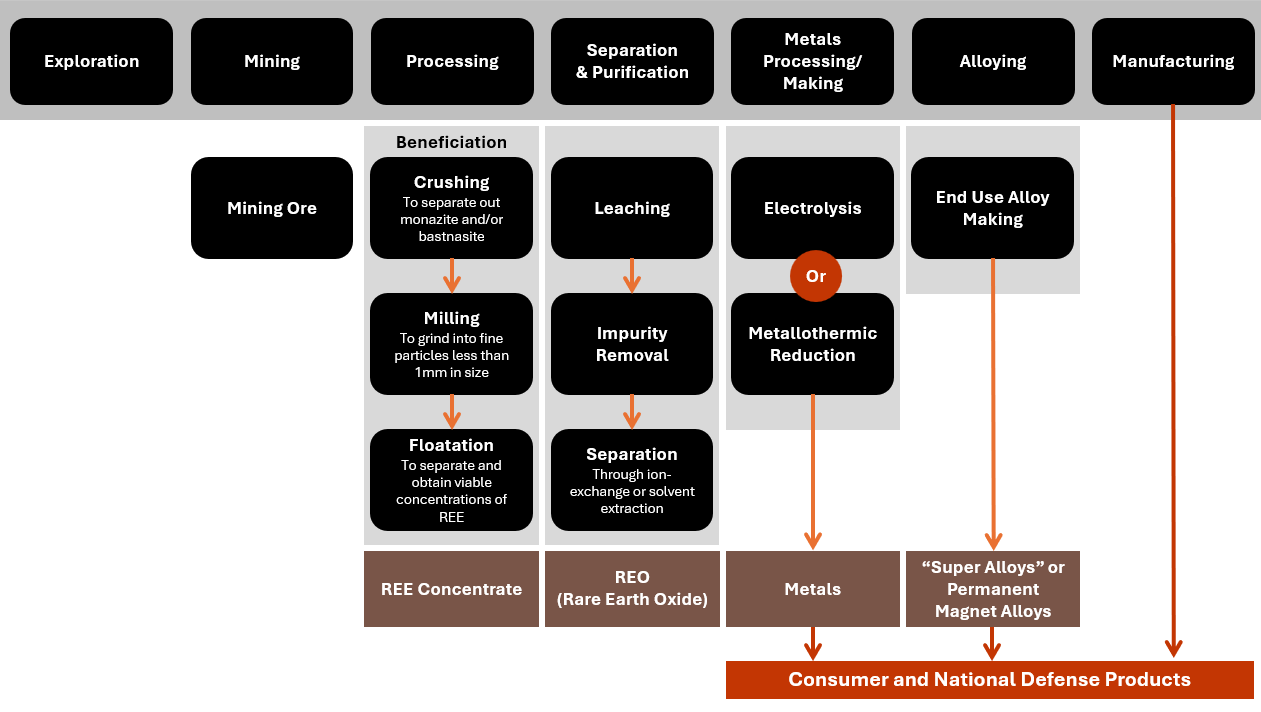
\includegraphics[width=1\linewidth]{Final_report_files/figure-latex/Critical_Mineral_Extraction_Process_v2} 

}

\caption{REE Value Chain (Source: US Department of Energy, 2017)}\label{fig:ree-vc}
\end{figure}

Recently, water-leaching is a prevailing approach since it mitigate the flaw from traditional techniques. Water leaching can be considered as less environmentally detrimental compared to strong acid/alkaline leaching, as well as cost effective for solvent selection. The crucial stages on this preparation workflow are low temperature activation and water leaching. During the stage of low temperature activation, the chemical reaction within coal fly ash (CFA) will be facilitated by complexation agents (ammonium salts or weak acids) in covered alumina crucibles, which help liberate critical elements from the matrix of the CFA. After the activation and cool down to ambient temperature, the tablets are placed in water for the leaching and dissolve process. Water acts as the leaching solvent, extracting these soluble elements into the leachate.The configuration in temperature and mass ratio of solvent will be the vital determinant for optimized recovery. Take Lithium example, it can achieve a stable leaching efficiency of 90\% through ammonium fluoride leaching at 150°C with a \(SiO_2/NH_4F\) mass ratio of 1:1.35 \textcite{Xu2021}.

Another innovation is Hydrophobic-Hydrophilic Separation (HHS), designed to leverages the disparity of affinity (water-repellent \& water-friendly) properties of substances to achieve separation.It can treat as a complementary application for small particle delamination without size limit, providing flexible and extensible purpose in the segregation of ultrafine coal \textcite{Hodgkinson2021}.

In precious \textcite{Hodgkinson2020} element mapping project on Bowen basin,the largest coal reserves in Australia, the concentration of element composition is subjective to sample's lithology rather than the depth grading:

1). In coal and derivative, albeit majority of element concentrations is inferior of the benchmark against earth crust average, local samples exhibit enrichment in HREE and Scandium in respect to \textcite{McLennan2011} Post-Archaean Australian Shales (PAAS) standard , while abnormal 4-6 times higher than crustal average in moderate critical element, Bismuth(Bi) .

2). Siltstone and mudstone has a lackluster finding to classify enrichment for majority of elements concentration,except for the concentration of Cobalt compound barely meet crustal average, whose ubiquitous economic value may warrant further examination.

3). As the sediment from volcanic ash, tuffaceous rock is rich in pumice and lithic fragments. The sample display a series of elevated concentrations of strategic elements including REE, Ga and Bi. Besides, a potential Lithium-rich borehole is found, with approximate 5 times higher than crustal average.

\section{Objectives and Significance}\label{objectives-and-significance}

The primary objective of this study is to develop a predictive model using machine learning and spatial statistics to identify and quantify critical minerals---such as copper, lithium, nickel, cobalt, and rare earth elements---in coal mine waste. By analyzing existing coal data, this study aims to provide valuable insights into the potential recovery of these essential minerals from coal deposits, contributing to waste reduction and supporting the transition to low-emission technologies. The outcome of this study will help assess the economic value of these minerals and promote sustainable practices within the mining and energy sectors.

The study utilises multiple datasets, some of which are publicly available while others are confidential. The public dataset was released by the Australian Coal Industry's Research Program (ACARP) in 2021, whereas the confidential data comes from Matrix Geoscience's clients. Although the datasets originate from different sources, both contain information on the concentration of various critical elements sampled from coal mines and power plants across Australia. Additionally, the study employs data on elemental concentrations from Post Archean Australian Shale (PAAS), which represents the background crustal abundance of elements. This comparison helps determine whether the elemental concentrations in the coal samples exceed typical crustal abundance levels.

This study is significant because it addresses a critical gap in understanding the presence and potential recovery of valuable minerals from coal mine waste. By employing advanced machine learning and spatial statistics techniques, the project has the potential to revolutionise how the mining industry views coal waste---transforming it from an environmental challenge into a resource opportunity. The findings could contribute to more sustainable mining practices, reduce waste, and support the global transition to low-emission technologies by securing a local supply of critical minerals. Furthermore, this research could pave the way for further exploration of coal mine waste as a valuable resource in other regions, creating economic and environmental benefits on a broader scale.

\section{Data}\label{data}

\subsection{Data source and description}\label{data-source-and-description}

As the escalating research into this flourishing market, the largest national scientific research institution, CSIRO (Commonwealth Scientific and Industrial Research Organisation) in Australia Federation has initiated the early-stage research into the potential of element extraction in coal mines. Launched in 2001, The C29030 project in Australian Coal Industry's Research Program (ACARP) \autocite{Hodgkinson2021} has gauged the first comprehensive map of element concentration in Australian coal and provided the open dataset for testing result. This element mapping targets on 50 elements that has rarely studied from nearly 90 samples in Queensland and New South Wales, which are carefully selected in 13 coal mines and power plants to represent 6 basins, covering a range of coal measures and seams of varying ages. The dataset is a wide format excel spreadsheet, with the information of detected element name and their corresponding concentration in parts per million (ppm) for each labelled sample(e.g.2648CR01), as well as the sample's coordinate in a separate record.

Simultaneously, private-sector analyses are also promptly emerging, utilising a variety of advanced analytic techniques, including four-acid digestion with ICP-AES and fusion-based acid digestion with ICP-MS. Although the report format is not standardised (long or wide format), but all of them cover basic information for element name and concentration as well as additional borehole composite index in ppm, which is sufficient for further deep-dive investigation.

Eventually, PAAS file attached to \autocite{McLennan2011} Post-Archean Australian Shale normalised score, representing the average composition of shale formed after the Archean eon, which is a geochemical reference baseline in the comparison of element enrichment in this report.

\subsection{Initial Data Analysis and wrangling process}\label{initial-data-analysis-and-wrangling-process}

To prepare for exploratory data analysis and predictive modeling, different data formats must be collated into a standardised structure, which involves converting the data into a long format and trimming the trivial variables to ensure consistency and readiness for further analysis. The cleaning data will include \texttt{element\ symbol}, \texttt{elment\ value\ in\ ppm} and \texttt{project\ region} only, but other specific cleaning requirements still need to be addressed. First and foremost, The private projects are unable to disclose the location in detail, therefore; they will be replaced to Confidential A, B and C respectively. Furthermore, partial element values are recorded as character due to their undetected status(nd) and subtle presence(\texttt{\textless{}} sign). a value of \texttt{-999.00} will be assigned to represent their negative relationship without compromising data integrity. Another significant issue in data wrangling is the sample duplication, mainly because cross detection methods are applied in their analysis. To resolve this, we will remain the element concentration value for the most precise observation range.

After the preliminary tidying, the data is organised and concise but some information is still lacking in subsequent study. Since the analytic technique will only detect single element, the critical element groups like REE and it's subcategories are absent in calculation. the element list need to be expanded by the aggregation of the concentration values from their corresponding symbols. Additionally, the data must be joined with PAAS file and normalised value should be derived by using formula \(\text{Normalized value}= \frac{\text{Element value(ppm)}}{\text{PAAS score(ppm)}}\), along with Boolean flag for enrichment (above background, \textgreater=1). The final step is replacing outliers and missing values by the median value within their respective project. If no project-specific values are available the global median of the element will be applied. The median replacement is a mild imputation to ensure the robustness and consistency of data structure and in turn, maintain data integrity without distorting the subsequent modelling.

In a nutshell, The final cleaning data include total 8 variables and 11032 observations. Figure \ref{fig:visdat} shows the correct data type for all variables, with no missing value left.

\begin{figure}
\centering
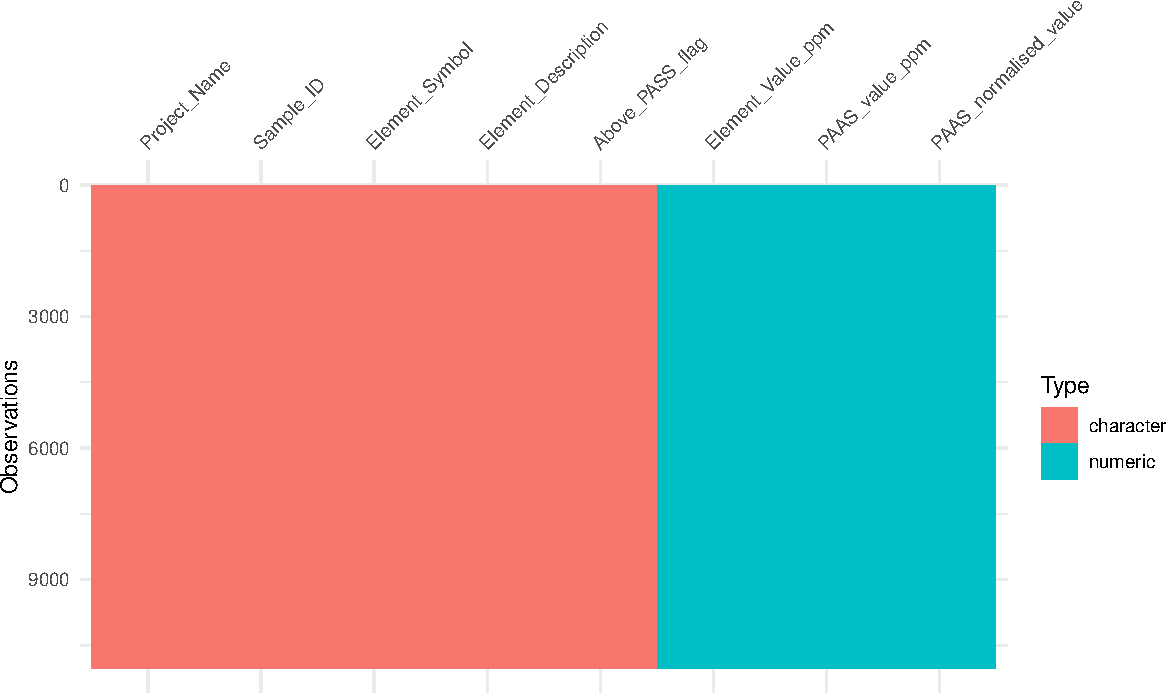
\includegraphics{Final_report_files/figure-latex/visdat-1.pdf}
\caption{\label{fig:visdat}n at-a-glance of final data wrangling result}
\end{figure}

\section{Exploratory Data Analysis}\label{exploratory-data-analysis}

The Exploratory Data Analysis (EDA) was carried out on critical elements concentration data, which provide information about the concentration of critical mineral across different areas in Australia that has been normalised using PAAS (Post-Archean Australian Shale) standard. The primary objective of this analysis is to gain a deeper understanding of the data's structure and key characteristics. Through this, we aim to identify significant trends, correlations, and outliers that may influence the outcomes of the study.

The EDA for critical elements concentration data starts with a descriptive statistics for every critical elements included in the data. These summary statistics can be found in the Table \ref{tab:desc-stats}. The descriptive statistics features include the minimum value of the critical elements, maximum value, the mean, the median, the standard deviation, and the kurtosis of the variable.

\begingroup\fontsize{9}{11}\selectfont

\begin{longtabu} to \linewidth {>{\centering}X>{}c>{\centering}X>{\centering}X>{\centering}X>{\centering}X>{\centering}X>{\centering}X}
\caption{\label{tab:desc-stats}\textbf{Descriptive Statistics of Elements' Normalised Value}}\\
\toprule
Element Symbol & Element Description & min & max & mean & median & sd & kurtosis\\
\midrule
\endfirsthead
\caption[]{\label{tab:desc-stats}\textbf{Descriptive Statistics of Elements' Normalised Value} \textit{(continued)}}\\
\toprule
Element Symbol & Element Description & min & max & mean & median & sd & kurtosis\\
\midrule
\endhead

\endfoot
\bottomrule
\endlastfoot
Ag & Silver & 2.000 & 13.200 & 4.142 & 3.600 & 2.389 & 5.783\\
Al & Aluminium & 0.000 & 8.500 & 0.845 & 0.438 & 0.982 & 34.192\\
Au & Gold & 0.556 & 12.222 & 3.521 & 3.333 & 2.064 & 7.764\\
Ba & Barium & 0.013 & 18.182 & 1.108 & 0.750 & 2.027 & 43.446\\
Be & Beryllium & 0.033 & 6.000 & 1.126 & 0.667 & 1.134 & 7.156\\
\addlinespace
Bi & Bismuth & 0.787 & 25.197 & 3.685 & 2.402 & 3.302 & 17.818\\
Cd & Cadmium & 0.102 & 7.347 & 1.271 & 0.918 & 1.115 & 9.839\\
Ce & Cerium & 0.056 & 5.938 & 0.956 & 0.985 & 0.595 & 21.060\\
Co & Cobalt & 0.118 & 7.882 & 0.906 & 0.588 & 1.133 & 17.661\\
Cr & Chromium & 0.012 & 10.807 & 0.441 & 0.205 & 1.048 & 54.642\\
\addlinespace
Cs & Caesium & 0.024 & 6.870 & 1.068 & 0.923 & 0.910 & 12.858\\
Cu & Copper & 0.040 & 10.200 & 1.681 & 1.880 & 1.160 & 13.140\\
Dy & Dysprosium & 0.114 & 5.286 & 1.522 & 1.517 & 0.847 & 5.566\\
Er & Erbium & 0.087 & 4.957 & 1.401 & 1.320 & 0.815 & 6.383\\
Eu & Europium & 0.114 & 7.773 & 1.676 & 1.648 & 0.969 & 8.535\\
\addlinespace
Fe & Iron & 0.000 & 9.689 & 0.474 & 0.180 & 1.066 & 45.053\\
Ga & Gallium & 0.076 & 3.076 & 1.293 & 1.291 & 0.684 & 2.148\\
Gd & Gadolinium & 0.132 & 6.605 & 1.589 & 1.513 & 0.901 & 7.420\\
Ge & Germanium & 0.088 & 43.750 & 7.481 & 0.344 & 13.031 & 3.653\\
HREE & Ho+Er+Tm+Yb+Lu & 0.036 & 0.995 & 0.282 & 0.267 & 0.157 & 6.712\\
\addlinespace
Ho & Holmium & 0.125 & 4.750 & 1.352 & 1.306 & 0.767 & 5.962\\
In & Indium & 0.400 & 7.200 & 1.434 & 1.000 & 1.117 & 9.581\\
LREE & La+Ce+Pr+Nd+Pm+Sm & 0.089 & 4.214 & 1.020 & 1.064 & 0.540 & 6.992\\
La & Lanthanum & 0.100 & 2.540 & 0.871 & 0.930 & 0.480 & 2.566\\
Li & Lithium & 0.250 & 14.250 & 2.386 & 2.000 & 1.974 & 9.533\\
\addlinespace
Lu & Lutetium & 0.000 & 6.250 & 1.540 & 1.438 & 0.919 & 7.067\\
MREE & Eu+Gd+Tb+Dy+Y & 0.088 & 4.384 & 1.361 & 1.344 & 0.756 & 5.952\\
Mn & Manganese & 0.002 & 18.717 & 0.594 & 0.109 & 1.884 & 66.528\\
Mo & Molybdenum & 0.067 & 13.733 & 2.971 & 2.667 & 2.195 & 10.237\\
Nb & Niobium & 0.042 & 3.567 & 0.622 & 0.647 & 0.402 & 16.601\\
\addlinespace
Nd & Neodynium & 0.065 & 4.423 & 1.145 & 1.221 & 0.645 & 4.693\\
Ni & Nickel & 0.023 & 8.182 & 0.386 & 0.159 & 0.869 & 44.099\\
Pb & Lead & 0.052 & 4.909 & 1.276 & 1.235 & 0.856 & 6.139\\
Pr & Praseodymi & 0.056 & 4.704 & 1.033 & 1.092 & 0.596 & 7.452\\
REE & La+Ce+Pr+Nd+Sm+Eu+Gd+Tb+Dy+Ho+Er+Tm+Yb+Lu & 0.134 & 4.174 & 1.089 & 1.130 & 0.539 & 6.574\\
\addlinespace
REEY & La+Ce+Pr+Nd+Sm+Eu+Gd+Tb+Dy+Ho+Er+Tm+Yb+Lu+Y & 0.138 & 3.641 & 1.120 & 1.151 & 0.528 & 4.600\\
Rb & Rubidium & 0.001 & 2.670 & 0.472 & 0.441 & 0.396 & 5.920\\
Re & Rhenium & 0.000 & 7.500 & 4.286 & 5.000 & 3.134 & 1.792\\
Sc & Scandium & 0.162 & 4.985 & 1.137 & 1.191 & 0.610 & 8.482\\
Sm & Samarium & 0.089 & 4.689 & 1.421 & 1.460 & 0.785 & 4.173\\
\addlinespace
Sn & Tin & 0.182 & 2.364 & 0.726 & 0.655 & 0.350 & 6.862\\
Sr & Strontium & 0.006 & 4.571 & 0.955 & 0.916 & 0.608 & 6.965\\
Ta & Thallium & 0.133 & 4.000 & 0.865 & 0.920 & 0.482 & 14.453\\
Tb & Terbium & 0.156 & 4.578 & 1.378 & 1.359 & 0.760 & 5.576\\
Th & Thorium & 0.044 & 5.329 & 1.172 & 1.107 & 0.853 & 6.382\\
\addlinespace
Tl & Tantalum & 0.030 & 10.000 & 1.942 & 0.715 & 3.123 & 5.782\\
Tm & Thulium & 0.303 & 5.455 & 1.453 & 1.364 & 0.816 & 7.679\\
U & Uranium & 0.054 & 4.286 & 1.289 & 1.304 & 0.805 & 3.219\\
V & Vanadium & 0.019 & 4.299 & 1.038 & 1.103 & 0.666 & 5.959\\
Y & Yttrium & 0.045 & 4.568 & 1.278 & 1.250 & 0.764 & 6.443\\
\addlinespace
Yb & Ytterbium & 0.091 & 5.409 & 1.462 & 1.400 & 0.854 & 6.361\\
Zn & Zinc & 0.014 & 4.324 & 0.921 & 0.930 & 0.699 & 4.134\\
Zr & Zirconium & 0.021 & 4.821 & 0.923 & 0.979 & 0.592 & 9.671\\*
\end{longtabu}
\endgroup{}

The most important statistics from this table is kurtosis. Kurtosis measures the combined weight of the tails of a distribution relative to its centre. In this way, we can use kurtosis as an indicator of the presence of outliers. A high kurtosis values is indicative of outliers. The summary statistics suggest that Al, Ba, Bi, Ce, Co, Cr, Cs, Cu, Fe, Mn, Nb, and Ni are having many outliers due to high kurtosis value. Validating the outliers will be easier with data visualisation, which will be presented in the next step.

The next step was analysing the distribution of each element's normalised value. By utilising boxplots, it will help identifying the outliers of each critical elements, while also identifying which element's has median value above the PAAS standard. Obtaining these information will help to understand whether certain element is naturally abundance in the nature, thus it is most likely economically efficient to extract. The figure \ref{fig:element-dist} provide these informations.

\begin{figure}

{\centering 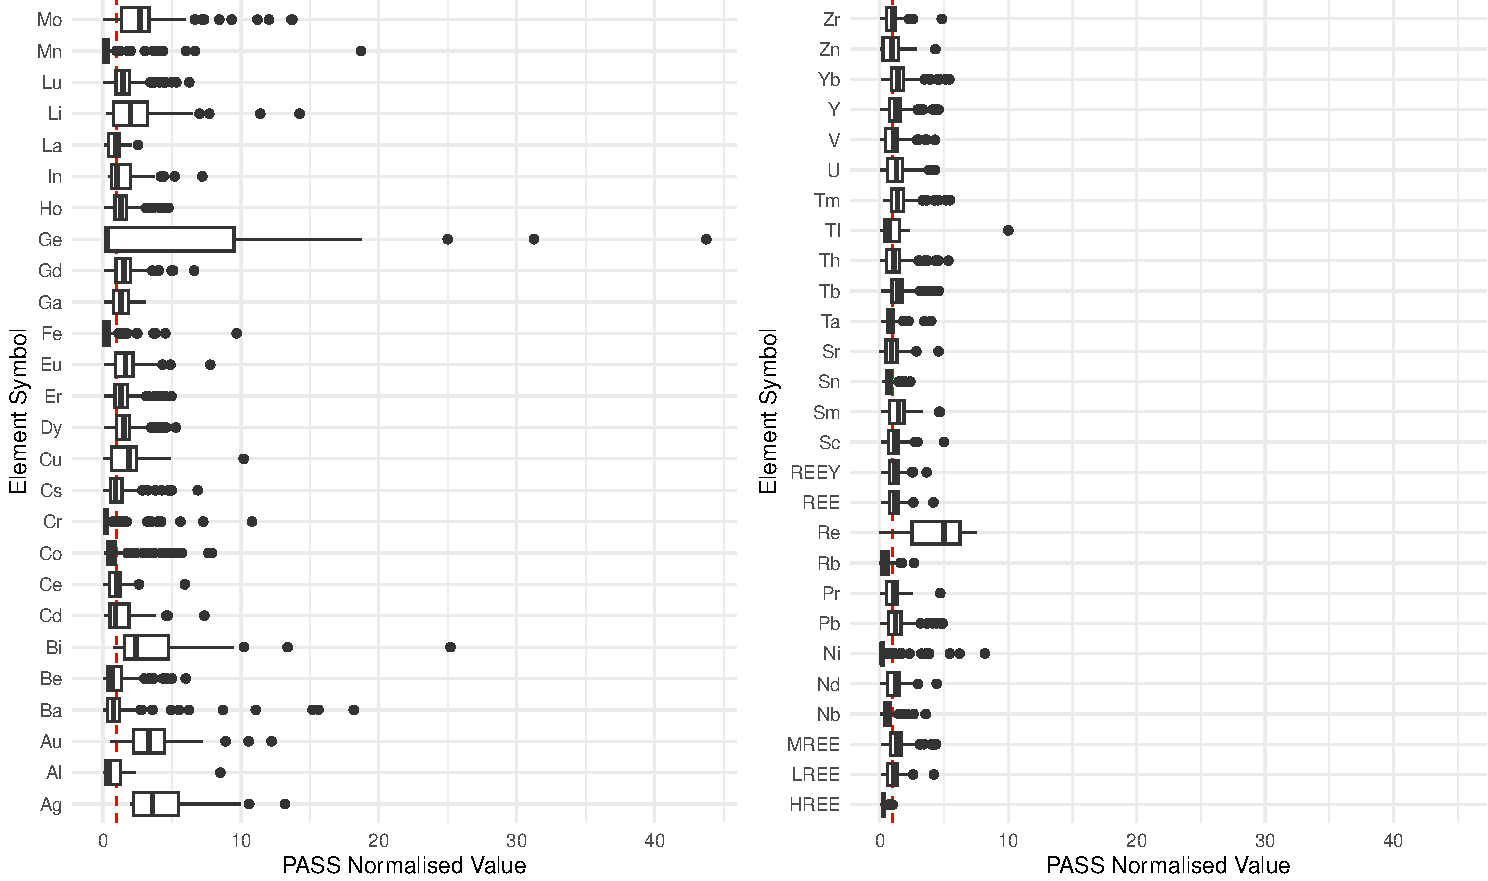
\includegraphics[width=1\linewidth]{Final_report_files/figure-latex/element-dist-1} 

}

\caption{Distribution of Critical Elements (Box-Plot)}\label{fig:element-dist}
\end{figure}

The boxplots shows some critical points that can be summarised as follow:

\begin{itemize}
\tightlist
\item
  Medians: Most of the elements have their medians close to 0, indicating that the majority of the values are low or concentrated around a lower range. Considering that the threshold to define whether a sample is below/above background is 1 (vertical red dashed line), some elements that have median above the threshold are Re, Ag, Au, Mo, Bi, Li, Cu, Eu, Dy, Gd, Sm, Lu, Yb, Tm, Tb, MREE, Er, Ho, U, Ga, Y, Pb, Nd, Sc, REEY, REE, Th, V, Pr, LREE
\item
  Spread and Variability: The elements exhibit varying degrees of spread. For example, Ge shows a wide range with its box stretching from a low value near 0 to a higher value around 10, indicating a large variability. On the opposite side, elements like Mn, Fe, Cr, Co, Rb, Ni, HREE have very narrow IQR, indicating less variability.
\item
  Outliers: Several elements have significant outliers, as indicated by the dots outside the whiskers of the box plots. For instance, Ge, Bi, Mn, and Ba show notable outliers far from the main data range. Additionally, some elements that was reported from table \ref{tab:desc-stats}, which have high kurtosis are Al, Ba, Bi, Ce, Co, Cr, Cs, Cu, Fe, Mn, Nb, and Ni. These outliers suggest the presence of some unusually high or low values for these elements, which could be of interest for further investigation.
\item
  Symmetry and Skewness: Some elements like Ge, Bi, and Ag appear to have a right skew, with longer whiskers or outliers extending to the right, indicating that the distribution of their normalised values has a tail on the higher end. Elements like Ga and Sm show a more symmetrical distribution with whiskers extending fairly equally on both sides of the box.
\item
  Comparison Accross Elements: Ge stands out with a particularly large spread and median, making it an outlier among the elements. Conversely, many rare earth elements (REE, REEY, MREE, LREE, HREE) have relatively low medians and a small spread, indicating that their normalised values are generally low and clustered.
\end{itemize}

\section{Methodology}\label{methodology}

\subsection{Predicting Critical Elements}\label{predicting-critical-elements}

The predictive modeling process in this project follows a structured methodology, consisting of key steps aimed at selecting the most accurate and robust model for predicting the target variable. Each step contributes to refining the model's performance, from data preprocessing and feature selection to model training and evaluation. The overall framework of this methodology is outlined in the figure \ref{fig:modelbuilding}.

\begin{figure}
\centering
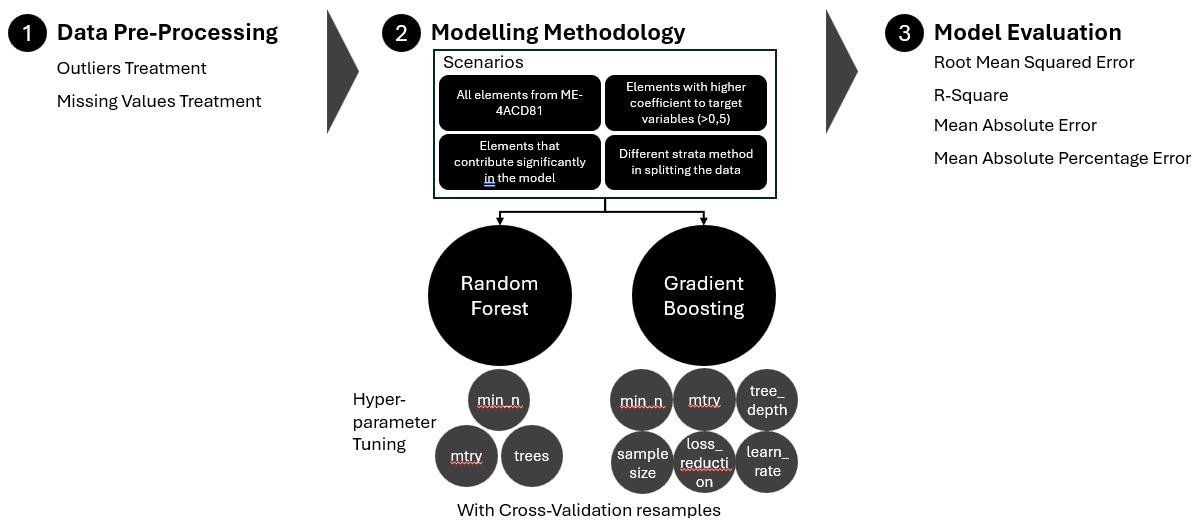
\includegraphics{Final_report_files/figure-latex/Methodology.png}
\caption{\label{fig:modelbuilding}The mindset of model build-up in predictive analysis}
\end{figure}

The methodology for this study follows a three-stage process. First, data preprocessing is conducted, addressing outliers and missing values to ensure clean data. Next, several modeling scenarios are explored using Random Forest and Gradient Boosting, with hyperparameter tuning applied to optimise model performance. These scenarios include using all elements, elements with high correlation to target variables, and different stratification methods for data splitting. Finally, model performance is evaluated using key metrics such as Root Mean Squared Error (RMSE), R-squared, Mean Absolute Error (MAE), and Mean Absolute Percentage Error (MAPE).

\subsubsection{Data Pre-Processing}\label{data-pre-processing}

On one hand, outlier is well known as the observations/data points that deviate significantly from other observations in a dataset. On the other hand, missing value is observation when there is no data stored for certain variables. In predictive modelling, outliers and missing value can have an effect to the regression model when predicting the target variable in a negative way. For example, outliers value will disrupt the normal pattern of the dataset, while missing value will introduce uncertainty to the model. Thus, if not treated, they might lead the model to make inaccurate predictions. With this concern, outlier and missing value will be treated, aimed to reduce the negative effect to the model performance.

For outlier, Tukey! introduce the approach to detect outlier in a dataset. He defined that outlier can be detected by the 1.5 Interquartile Range (IQR). An observation is considered an outlier if it lies below Q1 - 1.5xIQR or above Q3 + 1.5xIQR, where IQR is the interquartile range between the first and third quartiles. This method is particularly effective for detecting outliers in data with a skewed distribution. This method will be applied to the dataset for this project in detecting outliers. Next, in treating the outliers, {[}Barnett{]} stated that, as a simple approach, outliers can be replaced with sample median for robust estimation. This, with the additional issue regarding lab test error in determining the elements' concentration values, the outliers will be replaced with median value of where the samples were obtained from. For example, for outliers detected in ``Sc'' data from ``Confidential Project A'', then those outliers will be replaced with median value of ``Sc'' of ``Confidential Project A''.

For missing values, Hastie! stated that, there are number of ways in treating missing value (assuming random missing value), which are remove observations with any missing value; rely on the learning algorithm to handle missing values during the training process; and fill in all missing values prior to training process. The last option was chosen and the missing value are filled with the median value of where the samples were obtained from, but if the element does not exist in that particular project, then the global median will be applied. For example, for missing value detected in ``Sc'' data from ``Confidential Project A'', then those missing values will be replaced with median value of ``Sc'' in general.

\subsubsection{Stratified sampling and Initial split}\label{stratified-sampling-and-initial-split}

Unlike simple random sampling, stratified sampling is deployed to preserve the diversity of project's key feature across the training and test datasets, which leads to unbiased predictive modeling. However, some projects have limited borehole samples measured in the laboratory and their patterns might not be adequately presented in the initial data split. Thus, the project-based aggregation in terms of the classification within correlation matrix offers an effective solution to mitigate this bias. To properly address the hidden pattern in the neighbor similarity against global matrix, The approach incorporates completed pairwise method to neglect NA in correlation calculation and all element in the list {[}Menon2020{]}. Based on this strata division, the raw data will be split to training and testing set with 2/3 proportion.

\subsubsection{Prediction Model}\label{prediction-model}

In this project, the tidymodels package will be used to implement predictive modeling in R. Tidymodels is a comprehensive framework built on tidyverse principles, designed for modeling and machine learning {[}tidymodels{]}. Two prediction methods are employed in this analysis: Random Forest (RF) and Gradient Boosting Tree (GBT), both of which are well-suited for handling complex, non-linear relationships in the data. These methods have been selected for their robustness in prediction and their ability to minimise overfitting through ensemble learning techniques.

Random Forest is an ensemble learning method that constructs multiple decision trees using subsets of the training data through a technique called `bagging' (Bootstrap Aggregating). Bagging is a variance reduction technique for an estimated prediction function. In regression, this involves fitting the same regression tree multiple times to different bootstrap samples of the training data and averaging the results. Random Forest is a significant modification of bagging, as it builds a large collection of de-correlated trees and then averages their outputs. The concept behind Random Forest is to improve the variance reduction achieved by bagging by reducing the correlation between the trees, while minimizing any increase in variance. This is accomplished by randomly selecting input variables during the tree-growing process {[}Hastie; breiman{]}. The engine setting in tidymodels will be set to \texttt{randomForest}.

Whereas random forests build an ensemble of deep independent trees, GBT build an ensemble of shallow trees in sequence with each tree learning and improving on the previous one. The main idea of boosting is to add new models to the ensemble sequentially. In essence, boosting attacks the bias-variance-tradeoff by starting with a weak model (e.g., a decision tree with only a few splits) and sequentially boosts its performance by continuing to build new trees, where each new tree in the sequence tries to fix up where the previous one made the biggest mistakes (i.e., each new tree in the sequence will focus on the training rows where the previous tree had the largest prediction errors) {[}Boehmke github{]}. The engine setting in tidymodels will be set to \texttt{xgboost}.

\subsubsection{Hyperparameter tuning}\label{hyperparameter-tuning}

Building an effective machine learning model is a complex and time-intensive process that requires selecting the appropriate algorithm and optimizing the model's architecture through hyperparameter tuning. Machine learning models have two kinds of parameters: model parameters, which are initialised and updated during the training process (such as weights in neural networks), and hyperparameters, which cannot be learned from the data and must be set before training begins. Hyperparameters define key aspects of the model's structure and learning process. Examples include the penalty parameter in support vector machines, the learning rate in neural networks, the activation function, and optimizer types. Hyperparameter tuning is essential for improving model performance, as it involves finding the optimal combination of settings that maximises predictive accuracy {[}Yang{]}. Tree-based model have more hyperparameter that can be tuned, however, for this project, seven key hyperparameters were the top priority for tuning, which are:

1). mtry (number of predictors to sample): Controls the number of predictors considered at each split in a decision tree. A smaller mtry introduces more variability among trees, while a larger mtry can lead to more accurate splits but risks in overfitting problem.

2). min\_n (minimal terminal node size): Determines the minimum number of observations in the ending node. Smaller values allow trees to grow deeper, capturing more details in training data, while larger values lead to simpler models that may generalize better.

3). trees (number of trees): Define the the total number of decision trees in the ensemble. More trees generally improve performance but also increase computational cost.

4). tree\_depth (tree depth): Controls the depth of the individual trees.

5). learn\_rate (learning rate): It determines the influence of each tree on the final prediction and regulates the pace at which the algorithm progresses along the gradient descent path (or learns).

6). sample\_size (Number of Trees): Define the the total number of decision trees in the ensemble. More trees generally improve performance but also increase computational cost.

7). loss\_reduction (Number of Trees): The reduction in the loss function required to split further

To determine the best combination of these hyperparameters in the grid, k-fold cross-validation was employed. In k-fold cross-validation, the dataset is randomly divided into K equal-sized groups, known as ``folds.'' For each resampling iteration, the model is trained on K-1 folds, while the remaining fold is used for validation. In standard k-fold cross-validation (without repetition), the process is repeated \emph{K} times, ensuring that each fold is used once for validation {[}tidymodels{]}. Cross-validation provides a reliable estimate of the optimal tuning parameter value.

\subsubsection{Model evaluation}\label{model-evaluation}

When assessing a model's performance on a particular dataset, it is essential to have a method for determining how closely its predictions align with the actual observed data. This involves measuring the degree to which the predicted value for an observation approximates the true value for that observation. In this project, several metrics will be used, including Root Mean Squared Error (RMSE), Mean Absolute Error (MAE), Mean Absolute Percentage Error (MAPE), and R-Squared. These metrics provide a comprehensive understanding of how well the model fits the data, capturing both the average magnitude of error and the variability explained by the model {[}ISLR;Hastie{]}.

\paragraph{Root Mean Squared Error (RMSE)}\label{root-mean-squared-error-rmse}

RMSE is a standard way to measure the error of a model in predicting continuous outcomes. It represents the square root of the average of the squared differences between the observed and predicted values. RMSE gives more weight to large errors, making it particularly useful when large errors are undesirable {[}ISLR;Hastie{]}. The formula for RMSE is:

\(RMSE = \sqrt{\frac{1}{n} {\sum^n_{i=1}(y_i-\hat{y_i})^2}}\)

where \(y_i\) is the actual value, \(\hat{y_i}\) is the predicted value, and n is the number of observations.

\paragraph{Mean Absolute Error (MAE)}\label{mean-absolute-error-mae}

MAE measures the average magnitude of the errors in a set of predictions, without considering their direction. It's a linear score, meaning all individual differences are weighted equally {[}ISLR;Hastie{]}. The formula for MAE is:

\(MAE = \frac{1}{n} {\sum^n_{i=1}|y_i-\hat{y_i}|}\)

MAE is easy to interpret because it provides the average error in the same units as the target variable.

\paragraph{Mean Absolute Percentage Error (MAPE)}\label{mean-absolute-percentage-error-mape}

MAPE expresses the error as a percentage of the actual values, making it useful for comparing models on different scales or datasets. However, MAPE can be problematic when actual values are very close to zero {[}ISLR;Hastie{]}. The formula for MAPE is:

\(MAPE = \frac{100\%}{n} {\sum^n_{i=1}|\frac{y_i-\hat{y_i}}{y_i}|}\)

\paragraph{R-squared (Coefficient of Determination)}\label{r-squared-coefficient-of-determination}

R-squared explains the proportion of the variance in the dependent variable that is predictable from the independent variables. It provides insight into how well the model captures the variability in the data, with a higher R-squared indicating a better fit {[}ISLR;Hastie{]}.

\(R^2 = 1-\frac{\sum^n_{i=1}(y_i-\hat{y_i})^2}{\sum^n_{i=1}(y_i-\bar{y})^2}\)

where \(\bar{y}\) is the mean of the actual values.

\paragraph{Additional Considerations}\label{additional-considerations}

These evaluation metrics each have strengths and weaknesses. RMSE penalizes large errors more than MAE, making it more sensitive to outliers. MAPE is useful for interpretation as it gives a percentage error, but it can be misleading when actual values are very low. R-squared is a useful measure of fit, but it can sometimes be artificially high in overfitting scenarios. Therefore, it is essential to use a combination of these metrics to gain a well-rounded understanding of the model's performance. For this project, we are going to look for a model that produce the smallest RMSE, MAE, and MAPE, while produce the largest R-Squared, because this implies the model produce the least error and cover the most variability from the data.

\section{Results}\label{results}

\section{Discussions}\label{discussions}

\section{Conclusion}\label{conclusion}

\section{Appendix}\label{appendix}

\newpage

\printbibliography[title=Reference]

\end{document}
